\section{Stand der Technik}

Im folgenden werden zwei verschiedene Arten von Zahlungsverfahren analysiert und deren
Vorteile in Bezug auf Sicherheit und Härtungsmaßnahmen dargestellt: drahtlose Zahlung mit und 
Smartcards.

\subsection{Drahtlose Verbindungen und Sicherheit bei Bezahlungen}

Viele digitale Zahlungen finden über NFC statt. Diese Technologie ermöglicht ein Zahlungs- und
Identifizierungsverfahren, indem ein passives Gerät oder auch Tag genannt mit einem aktiven Gerät,
auch Ermittler genannt, kommuniziert. In dieser Situation will das passive Gerät eine Autorisierung initiieren,
während das aktive Gerät für die Erlaubnis zuständig ist \cite{refart:NFNK}. 

\begin{figure}[H]
   \centering{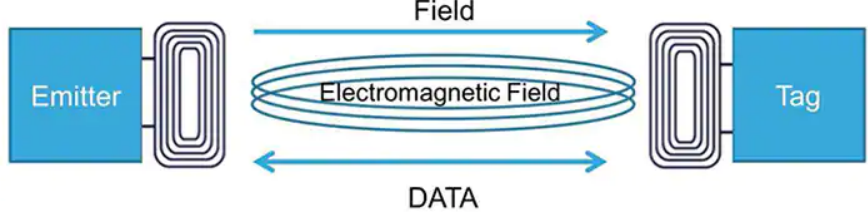
\includegraphics[width=8cm]{Bilder/refart_GPIN}}
   \caption{Teilnehmer der Kommunikation über \acrshort{nfc}\\Quelle: Proehl, 2021}
   \label{fig:refart_GPIN}
\end{figure}
% \cite{refart:GPIN}

\subsubsection{Angriffsmöglichkeit auf \acrshort{nfc}}

Da diese Technologie neu ist \cite{refip:NTAS}, sie existiert seit 2006, sind Schwachstellen 
und Härtungsmaßnahmen nicht in ihrer Vollständigkeit bekannt. Drahtlose Verbindungen sind auch für ihre 
Schattenseite bekannt \cite{refip:NYRS}. Maßnahmen zu entwickeln, die sich an verschiedene Systeme anpassen,
kosten Zeit und Investitionen von Banken und Sicherheitsfirmen. Für jeden möglichen Angriffe müssten 
Gegenmaßnahmen existieren, sodass das Schutzziel der Integrität\footnote{Es ist Subjekten nicht möglich, 
die zu schützenden Daten unautorisiert und unbemerkt zu manipulieren \cite{refbook:SWIS}.} nicht verletzt wird.

Bekannte Angriffe für drahtlose Verbindungen können auch bei \acrshort{nfc} verwendet werden\cite{refip:NYRS}, wie die
Erstellung und das Hinzufügen von Dateien in einem Opfersystem mit umfangreichen Privilegien; die Konzipierung
von schwachen digitalen Zertifikaten oder auch die Verwendung von Reverse Engineering\footnote{Reverse
Engineering ist ein Prozess von der Identifizierung von Bestandteilen eines Systems und von die Wiederherstellung 
dieser in einem anderen Format \cite{refart:CHRE}. Im Bereich der Cybersicherheit wird Reverse Engineering 
verwendet, um Schwachstellen von Systemen zu entdecken, sodass diese gegen Hardware und Software ausgenutzt
werden können \cite{refip:CMBM}.}. \cite{refart:ALSI} hebt andere Schwachstellen hervor: 
\textit{Eavesdropping}\footnote{Eavesdropping ist das unautorisierte Mithören von einer Kommunikation 
\cite{refbook:SWIS}.} je nachdem, wie viele Ressourcen investiert werden, kann ein Angreifer in der 
Lage sein, der Kommunikation zu lauschen; \acrfull{ddos}\footnote{Bei solchen Angriffen wird die
Verfügbarkeit des Dienstes verletzt, sodass die Kommunikation nicht mehr einwandfrei funktioniert \cite{refbook:SWIS}. 
In diesem Fall findet dieser Angriff mithilfe vieler Quellen statt, die von dem Angreifer ferngesteuert sind.},
um die Authentifizierung und Verfügbarkeit der Kommunikation zu beeinträchtigen.


\subsubsection{Gegenmaßnahmen für die Härtung von drahtlose Verbindung}

Um die Risiken bei der Verwendung von \acrshort{nfc} zu abzuschwächen, schlägt \cite{refip:NYRS} einige Sicherheitsmechanismen vor, 
die sich eher auf allgemeine drahtlose Verbindungen beziehen die aber auch für \acrshort{nfc} verwendet werden können: Nutzung
von modernen kryptographischen Standards für die Validierung von Zertifikaten; \acrfullpl{2fa} oder \acrfullpl{mfa}\footnote{\acrfullpl{2fa} oder \acrfullpl{mfa} bezeichnen das Authentifizierungsverfahren, indem zwei oder mehrere 
unabhängige Komponenten zur Authentifizierung verwendet werden, z.B. ein Passwort zusammen mit dem Fingerabdruck,oder eine Karte 
zusammen mit der Erkennung des Muster der Iris im Auge \cite{refip:simf}.}; Erstellung von schwer zu erratenden Passwörtern;
Registrierung von autorisierten Geräten; Einsetzung von \acrlong{ki}\footnote{\acrlong{ki} oder \acrlong{ai} im Original
bezeichnet das Verfahren, in dem Computer in der Lage sind, menschliche Entscheidung zu treffen\cite{refart:HAKI}. Ein Ziel
von \acrshort{ki} ist das menschliche Gehirn zu verstehen und in einer Maschine nachzubauen. Da die Definition nicht eindeutig 
ist und sich von viele andere wichtigen Wissenschaftler erklären lässt, verwenden hier für diese wissenschaftliche Arbeit die oben
genannte Definition.} für die Detektion von abweichendem Verhalten; Kontrolle gegen Social Engineering\footnote{Beim Social Engineering 
nutzt der Täter den ``Faktor Mensch'' als vermeintlich schwächstes Glied der Sicherheitskette aus, um seine kriminelle Absicht zu 
verwirklichen.\cite{booklet:BSSE}}

Kredit- und EC-Karten sollen auch als Zahlungsmittel bei unserem \acrshort{cba} akzeptiert werden. 
In Bezug auf diese Zahlungsmittel, wird die Sicherheit im folgenden untersucht.

\subsection{Anwendung von Smartcards und sicheres Bezahlen}
Smartcards sind heutzutage stark verbreitet im Bezug auf Zahlungsabwicklungen und auch für die Identifizierung.
Viele Ausweise, wie der Reisepass und die Krankenkassenkarte, verwenden diese Technologie zur Authentifizierung
des Nutzenden. In der folgenden Abbildung ist ein Beispiel von einer Smartcard für Zahlungsabwicklungen zu sehen: 

\begin{figure}[H]
   \centering{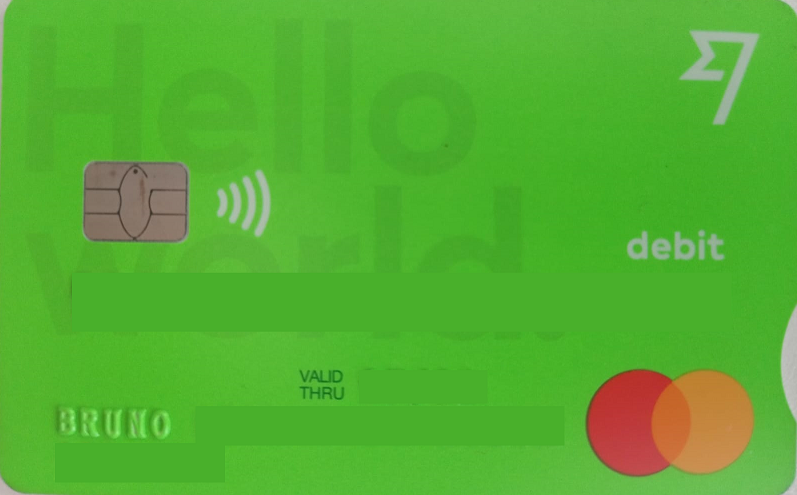
\includegraphics[width=4cm]{Bilder/eigenes_Bild_Karte.png}}
   \caption{Eine Smartcard und deren eingebettete Mikrochip\\Quelle: eigene Darstellung}
   \label{fig:eigenes_Bild}
\end{figure}

Die Smartcard wurde vor mehr als 40 Jahren erfunden und ihr Ziel ist die Sicherheit von Kartenzahlungen und 
allgemeine Authentifizierungsverfahren zu erhöhen \cite{refip:JFSB}. Sie unterscheiden sich von traditionellen 
Magnetstreifenkarten, weil sie verschiedene Authentifizierungsmethoden ermöglichen auch ohne eine direkte 
Verbindung zur Bank \cite{refbook:ATMS}. Im folgenden wird der Authentifizierungsprozess einer Smartcard 
\ref{fig:refbook_ATMS} dargestellt. 

\begin{figure}[H]
    \centering{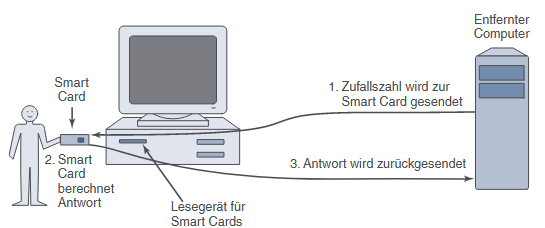
\includegraphics[width=6cm]{Bilder/refbook_ATMS.png}}
   \caption{Authentifizierungsprozess von Smartcards\\Quelle: Tanenbaum, 2009, S.755}
   \label{fig:refbook_ATMS}
\end{figure}

Die meisten Angriffe bei Smartcards geschehen laut \cite{refmas:ASSS} auf Hardwareebene. Er beschreibt folgende 
Techniken für Angriffe: Protokollanalyse, schwache Konzipierung oder mangelnde Verschlüsselung ermöglichen Zugang 
zum Klartext; Hardware Reverse Engineering: Verständnis über die Algorithmen oder Extrahieren des Schlüssels.


\subsubsection{Angriffsmöglichkeiten auf Smartcards}
Smartcards sind auf Hardwareebene extrem sicher. \cite{refmas:ASSS} bezeichnet sie auch als ein in Hardware gegossener
Tresor für Informationen. Wenn eine Smartcard für das Bezahlen verwendet wird, ist kein Backend-System nötig,
denn alle wichtigen Informationen wie das Guthaben sind direkt auf der Karte gespeichert. Aus diesem Grund können
keine Daten abgefangen werden, die auf dem Weg vom Lesegerät zum Backend-System sind, was den Bezahlprozess
deutlich sicherer macht \cite{refbook:WRHC}. Zudem muss jede Kommunikation vom Lesegerät initiiert werden, 
die Karte selber startet also keine Kommunikation. Da die wichtigsten Daten direkt auf der Karte gespeichert sind,
muss ein Angriff auf die Hardware initiiert werden, um an relevante Informationen zu gelangen. Eine weitere 
Möglichkeit wäre, die Schwachstellen eines bestimmten Protokolls, das für die Kommunikation verwendet wird auszunutzen.

\subsubsection{Gegenmaßnahmen für die Härtung von Smartcards}
Um einen Angriff auf die Hardware möglichst zu vermeiden, ist es sinnvoll den Chip nicht rekonstruierbar zu machen, d.h. dass
keine Standardzellen oder ähnliches verwendet werden. Zusätzlich spielt die Verschlüsselung der Daten eine große Rolle und 
erhöht die Sicherheit enorm \cite{refst:ARES}. Außerdem können Mechanismen in die Smartcard eingebaut werden, die permanent 
die Spannung oder Frequenz überprüfen und sobald etwas nicht dem Normalzustand entspricht, wird der Chip ausgeschaltet, sodass 
kein Lesegerät mit der Karte kommunizieren kann. Letztlich ist es wichtig, dass jede Karte individuell ist, sodass ein 
erfolgreicher Angriff kein Sicherheitsrisiko für andere Karten darstellt \cite{refmas:ASSS}. Dazu wären asymmetrische 
Verschlüsselungsverfahren\footnote{Bei asymmetrischer Verschlüsselung werden einen öffentlichen Schlüssel für die Verschlüsselung
und eine privaten Schlüssel für die Entschlüsselung der Daten verwendet \cite{refbook:SWIS}.} sinnvoller als 
symmetrische\footnote{Bei symmetrischer Verschlüsselung gibt es nur einen Schlüssel die sowohl für die Ver- als auch
für die Entschlüsselung der Daten verwendet wird\cite{refbook:SWIS}.}, da jede Karte bei asymmetrischer Verschlüsselung einen
öffentlichen und privaten Schlüssel hat und somit alle einen unterschiedlichen Schlüssel haben.


\subsection{Fazit}

NFC ist eine Technologie die viele Vorteile bietet. Sie ermöglicht in nur einem Gerät die Anwendung
verschiedener Aktivitäten, wie Zahlung, Identifizierung und Authentifizierung, ohne dass ein Nutzer 
unterschiedliche Karten bei sich haben muss. Die Nachteile beziehen sich auf die Neuigkeit dieser Technologie,
die mehr Forschung verlangt, damit deren Schwachstellen weiter erforscht werden \cite{refart:ALSI}. Die
Technologie der Smartcards ist bereits breit erforscht, sodass sowohl Schwachstellen, als auch Härtungsmaßnahmen
bekannt sind. Die Akzeptanz und die Verwendung von Smartcards sind auch größer, da besonders Non-Natives eher auf
Smartcards zurückgreifen.

Aus den obigen genannten Gründen können wir sagen, dass Smartcards der bessere Einsatz für einen \acrshort{cba}
neben einem Campingplatz wäre, solange die Technologie von NFC noch nicht so weit erforscht ist und in der 
Gesellschaft nicht so etabliert ist.
